\documentclass[border=10pt,varwidth]{standalone}
\usepackage[left=25mm,right=25mm,top=25mm,bottom=25mm]{geometry}
\usepackage[utf8]{inputenc}
\usepackage[T1]{fontenc}
\usepackage{times}
\usepackage{geometry}
\usepackage{amsmath}
\usepackage{amssymb}
\usepackage{mathrsfs}
\usepackage{amsfonts}
\usepackage{amsthm}
\usepackage{lipsum}
\usepackage{amscd}
\usepackage{graphicx}
\usepackage{fancyhdr}
\usepackage{textcomp}
\usepackage{txfonts}
\usepackage[all]{xy}
\usepackage{paralist}
\usepackage[colorlinks=true]{hyperref}
\usepackage{array}
\usepackage{tikz}
\usepackage{slashed}
\usepackage{pdfpages}
\usepackage{cite}
\usepackage{url}
\usepackage{amsmath,amsfonts,amssymb}
\usetikzlibrary{shapes.geometric}
\usepackage{tikz}
\usetikzlibrary{automata,positioning}
\usepackage{listings}
\usepackage{multirow}
\usepackage{color}
\usepackage{pgfplots}
\DeclareUnicodeCharacter{2212}{−}
\usepgfplotslibrary{groupplots,dateplot}
\usetikzlibrary{patterns,shapes.arrows}
\pgfplotsset{compat=newest}\begin{document}



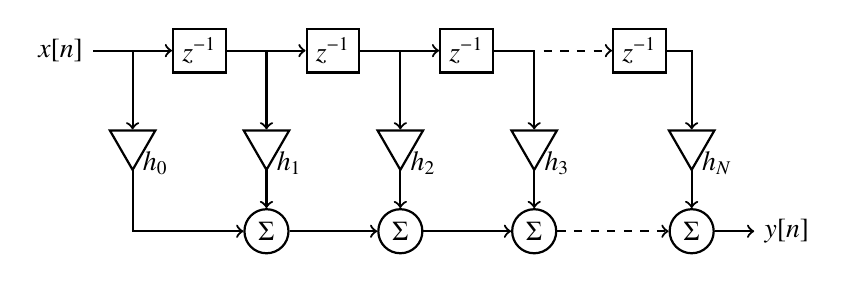
\begin{tikzpicture}

\draw[->,thick] node[anchor=east] {$x[n]$} (0,0) -- (1,0)
 node[anchor=west,draw,thick,minimum width=1,minimum height=1] (z1) {$z^{-1}$}  ;
\draw[->,thick] (z1.east) --++ (1,0)  node[anchor=west,draw,thick,minimum width=1,minimum height=1] (z2) {$z^{-1}$};
\draw[->,thick] (z2.east) --++ (1,0)  node[anchor=west,draw,thick,minimum width=1,minimum height=1] (z3) {$z^{-1}$};
\draw[thick] (z3.east) -- (5.6,0){};
\draw[->,thick, dashed] (z3.east) --++ (1.5,0) node[] (end) {};
\node[anchor=west,draw,thick,minimum width=1,minimum height=1] at (end) (z4) {$z^{-1}$};

\draw[->,thick] (0.5,0) -- (0.5,-1) node[isosceles triangle,
isosceles triangle apex angle=60,
draw, rotate=270, anchor=west,
minimum size=0.5cm] (t1) {} node[anchor=north west] at (t1) {$h_0$};
\node at (0.5,-1.5)  (test) {};
%  node[anchor=west,circle,draw,inner sep=2.5pt]{$\Sigma$};

\draw[->,thick] (2.2,0) -- (2.2,-1) node[isosceles triangle,
isosceles triangle apex angle=60,
draw, rotate=270, anchor=west,
minimum size=0.5cm] (t2) {} node[anchor=north west] at (t2) {$h_1$};
\draw[->, thick] (t2 |- test) --++ (0,-0.5) node[anchor=north,circle,draw,inner sep=2.5pt] (sigma) {$\Sigma$};

\draw[->, thick] (test.center) -- (test |- sigma) -- (sigma.west);

\draw[->,thick] (3.9,0) -- (3.9,-1) node[isosceles triangle,
isosceles triangle apex angle=60,
draw, rotate=270, anchor=west,
minimum size=0.5cm] (t3) {} node[anchor=north west] at (t3) {$h_2$};
\draw[->, thick] (t3 |- test) --++ (0,-0.5) node[anchor=north,circle,draw,inner sep=2.5pt] (sigma2) {$\Sigma$};

\draw[->, thick] (sigma.east) -- (sigma2.west);

\draw[->,thick] (5.6,0) -- (5.6,-1) node[isosceles triangle,
isosceles triangle apex angle=60,
draw, rotate=270, anchor=west,
minimum size=0.5cm] (t4) {} node[anchor=north west] at (t4) {$h_3$};
\draw[->, thick] (t4 |- test) --++ (0,-0.5) node[anchor=north,circle,draw,inner sep=2.5pt] (sigma3) {$\Sigma$};

\draw[->, thick] (sigma2.east) -- (sigma3.west);

\draw[thick] (z4.east) -- (7.613,0);

\draw[->,thick] (7.6,0) -- (7.6,-1) node[isosceles triangle,
isosceles triangle apex angle=60,
draw, rotate=270, anchor=west,
minimum size=0.5cm] (tn) {} node[anchor=north west] at (tn) {$h_N$};
\draw[->, thick] (tn |- test) --++ (0,-0.5) node[anchor=north,circle,draw,inner sep=2.5pt] (sigman) {$\Sigma$};

\draw[->, thick, dashed] (sigma3.east) -- (sigman.west);
\draw[->, thick] (sigman.east) --++ (0.5,0) node[anchor=west] {$y[n]$};

\end{tikzpicture}

\bigskip

    $$y[n] = h_0 x[n] + h_1 x[n-1]+\cdots + h_N x[n-N]$$

    $$ \mathbf{h} = [h_0, h_1, \dots, h_N]$$

    $$ y[n] = x[n] * h[n] $$

    $$y[n] = \sum^N_{i=0} h_i x[n-i]$$


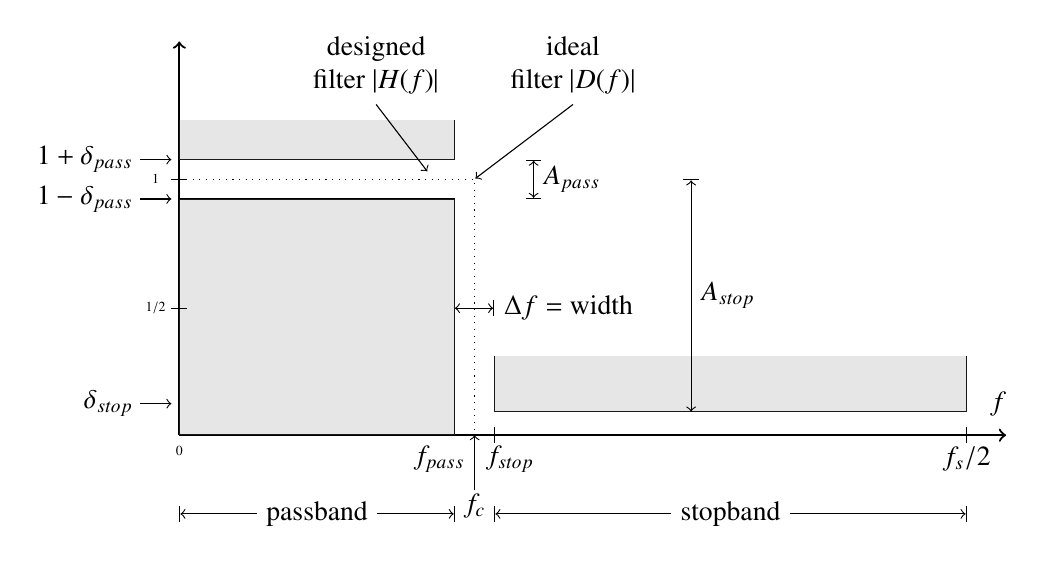
\begin{tikzpicture}
    \draw[->, thick] (0,0) -- (10.5,0);
    \draw[->, thick] (0,0) -- (0,5);
    
    \draw (0,3) -- (3.5,3) --++ (0,-3);
    \draw (0,3.5) -- (3.5,3.5) --++ (0,0.5);
    \fill[gray, fill opacity=0.2] (0,0) rectangle (3.5,3);
    \fill[gray, fill opacity=0.2] (0,3.5) rectangle (3.5,4);

    \draw (4,1) -- (4,0.3) -- (10,0.3) --++ (0,0.7);
    \fill[gray, fill opacity=0.2] (4, 0.3) rectangle (10,1);

    \draw[dotted] (0, 3.25) -- (3.75, 3.25) --++ (0,-3.25);
    
    \draw plot [smooth] file {../src/data.txt};
    
    \draw[->] (-0.5,3.5) -- (-0.1,3.5) node[yshift=0cm, xshift=-1.1cm] {$1+\delta_{pass}$};

    
    \draw[->] (-0.5,3) -- (-0.1,3) node[yshift=0cm, xshift=-1.1cm] {$1-\delta_{pass}$};
    \draw[->] (-0.5,0.4) -- (-0.1,0.4) node[yshift=0cm, xshift=-0.8cm] {$\delta_{stop}$};

    \draw[->] (2.5,4.2) node[above, align=center] {designed \\ filter $|H(f)|$} -- (3.15,3.35) ;
    \draw[->] (5,4.2) node[above, align=center] {ideal \\ filter $|D(f)|$} -- (3.76,3.26) ;

    \draw[-] (-0.1,3.25) -- (0.1,3.25) node[yshift=0cm, xshift=-0.4cm] {\tiny $1$};
    \draw[-] (-0.1,1.6125) -- (0.1,1.6125) node[yshift=0cm, xshift=-0.4cm] {\tiny $1/2$};

    \draw[<->|] (3.5,1.6125) -- (4,1.6125) node[right] {$\Delta f =$ width};
    \node at (0,-.2) {\tiny 0};

    \draw[->] (3.75,-0.7) -- (3.75,0) node[yshift=-0.9cm] {$f_c$};
    \draw[-] (3.5,--0.1) -- (3.5,0.1) node[xshift=-.2cm,yshift=-0.4cm] {$f_{pass}$};
    \draw[-] (4,-0.1) -- (4,0.1) node[xshift=0.2cm,yshift=-0.4cm] {$f_{stop}$};

    \draw[-] (10,-0.1) -- (10,0.1) node [xshift=0cm,yshift=-0.4cm] {$f_s/2 $};
    \node at (10,0)[xshift=0.4cm,yshift=0.4cm] {$f$};

    \draw[|<->|] (4.5,3) -- node[right] {$A_{pass}$} (4.5,3.5);
    \draw[<->|] (6.5,0.3) -- node[right] {$A_{stop}$} (6.5,3.25);

    \draw[|<->|] (0,-1) -- node[fill=white] {passband} (3.5,-1);
    \draw[|<->|] (4,-1) -- node[fill=white] {stopband} (10,-1);



\end{tikzpicture}


\end{document}
